\documentclass[11pt]{article}
\usepackage[margin=1in]{geometry}
\usepackage{amsmath,amssymb,amsthm,booktabs,graphicx,natbib,microtype}
\newtheorem{theorem}{Theorem}
\newtheorem{proposition}[theorem]{Proposition}
\newtheorem{corollary}[theorem]{Corollary}
\newtheorem{remark}[theorem]{Remark}
\newcommand{\norm}[1]{\left\lVert#1\right\rVert}
\newcommand{\wed}{\mathop{\bigwedge}\nolimits}
\title{The Global Wedge-Lipschitz Barrier\\\large A Sharp Negative Result for Fourth-Mode Support}
\author{Prime Dynamics Theory Program}
\date{July 2026}
\begin{document}
\maketitle
\begin{abstract}
We test a natural shortcut in finite-memory fourth-mode certification: perturb
the fourth exterior operator directly instead of perturbing four singular
values.  If $K=A+E$, $\norm{E}\leq\delta$, then
\[
 \norm{\wed^4K-\wed^4A}\leq(\norm A+\delta)^4-\norm A^4.
\]
The constant is sharp using only $\norm A$ and $\delta$.  We prove, however,
that the normalized lower certificate obtained from this inequality is
always dominated by the product Weyl certificate.  Its exact positivity
radius is $s_1((1+\widehat\nu_4)^{1/4}-1)\sim
s_1\widehat\nu_4/4$, compared with $s_4$ for product Weyl.  A 360-record
five-scale audit has zero domination failures and quantifies the loss.  This
is a negative result for global norm-only exterior perturbation, not for
directional wedge methods.
\end{abstract}

\section{Question and conclusion}
Let $s_1(A)\geq\cdots\geq s_r(A)$ and
\[
 \widehat\nu_4=\frac{s_1s_2s_3s_4}{s_1^4}.
\]
RH-109 used individual Weyl inequalities to propagate this normalized
four-volume through a finite-memory tail.  The global alternative is to view
$A\mapsto\wed^4A$ as one polynomial operator and apply a Lipschitz estimate.
The appeal is coordinate freedom.  The obstruction is that a norm-only
constant charges all four slots at $s_1$, erasing the weak-mode geometry.

Our conclusion is exact: the global method cannot improve product Weyl for
any spectrum or tail radius.  Since the global constant is itself sharp,
improvement requires directional or structured information.

\section{Sharp exterior perturbation law}
Exterior powers are understood as operators between the fourth exterior
spaces, equipped with their Hilbert norms \citep{HornJohnson1991}.

\begin{theorem}[Sharp global wedge perturbation]
Let $A,E$ be bounded operators between finite-dimensional Hilbert spaces and
$\norm E\leq\delta$.  For every positive integer $k$,
\begin{equation}\label{eq:lipschitz}
 \norm{\wed^k(A+E)-\wed^kA}
 \leq (\norm A+\delta)^k-\norm A^k.
\end{equation}
The right side cannot be reduced using only $\norm A$ and $\delta$.
\end{theorem}
\begin{proof}
Expand the alternating $k$-linear map into terms containing $j$ copies of
$E$.  There are $\binom{k}{j}$ such terms, each with norm at most
$\norm A^{k-j}\delta^j$.  Summing for $j\geq1$ gives
\eqref{eq:lipschitz}.  For $A=\alpha I$ and $E=\delta I$ on a $k$-space,
both exterior operators are scalar and equality holds.
\end{proof}

For $k=4$, write $a=s_1(A)$, $P=s_1s_2s_3s_4$, and
$R_4(a,\delta)=(a+\delta)^4-a^4$.  Since
$s_1(K)\leq a+\delta$, the global certificate is
\begin{equation}\label{eq:global}
 B_{\rm glob}=
 \frac{[P-R_4(a,\delta)]_+}{(a+\delta)^4}.
\end{equation}

\section{Weyl domination theorem}
The product certificate is
\begin{equation}\label{eq:weyl}
 B_{\rm Weyl}=\frac{\prod_{j=1}^4(s_j-\delta)_+}{(s_1+\delta)^4}.
\end{equation}

\begin{theorem}[Weyl domination theorem]\label{thm:domination}
For every nonincreasing nonnegative spectrum and every $\delta\geq0$,
\[
 0\leq B_{\rm glob}\leq B_{\rm Weyl}.
\]
\end{theorem}
\begin{proof}
If $\delta\geq s_4$, then $P\leq s_1^3\delta$ while
$R_4(s_1,\delta)\geq4s_1^3\delta$, so the global numerator is zero.
If $\delta<s_4$, telescope the loss produced by replacing each $s_j$ by
$s_j-\delta$.  Each of the four terms is at most $s_1^3\delta$, hence
\[
 P-\prod_{j=1}^4(s_j-\delta)\leq4s_1^3\delta
 \leq R_4(s_1,\delta).
\]
Rearrangement and the common denominator prove the claim.
\end{proof}

This theorem is stronger than a data-dependent comparison: it closes the
entire norm-only global route.

\section{Exact tolerance penalty}
The global numerator is positive precisely when
\[
 s_1^4\widehat\nu_4>(s_1+\delta)^4-s_1^4.
\]
Thus its maximal positive radius is
\begin{equation}\label{eq:radius}
 \delta_{\rm glob}=s_1\bigl((1+\widehat\nu_4)^{1/4}-1\bigr),
 \qquad \delta_{\rm Weyl}=s_4.
\end{equation}
For small four-volume,
$\delta_{\rm glob}=s_1\widehat\nu_4/4+O(\widehat\nu_4^2)$.
Because $\widehat\nu_4=(s_2/s_1)(s_3/s_1)(s_4/s_1)$, the global method
pays both the three-mode capacity and an additional factor near four.

\begin{remark}
Sharpness of \eqref{eq:lipschitz} does not say every fixed spectrum attains
the loss.  It says no theorem retaining only $\norm A$ and $\delta$ can
uniformly remove it.  A better route must preserve a frame, a tail Gramian,
or another directional datum.
\end{remark}

\section{Five-scale audit}
We reuse the finite-memory packets and outward-rounded tail radii archived in
RH-110.  The dataset has five scales, two channels, three thresholds, and
360 threshold-labelled records; 234 records lie on the three fine scales.
For every record we evaluate \eqref{eq:global}, \eqref{eq:weyl}, and the two
positivity radii in \eqref{eq:radius}.

\begin{table}[h]
\centering
\begin{tabular}{lrr}
\toprule
threshold & fine global support & fine product-Weyl support\\
\midrule
$10^{-8}$ & 72 & 78\\
$10^{-6}$ & 68 & 72\\
$10^{-4}$ & 55 & 55\\
\bottomrule
\end{tabular}
\caption{Certified fine updates out of 78 per threshold.  Values are filled
from the archived audit before release.}
\end{table}

There are zero domination failures and zero discrepancies with the archived
RH-110 product formula.  Figure~\ref{fig:audit} shows both the certificate
loss and the exact ratio of admissible positive radii.

\begin{figure}[h]
\centering
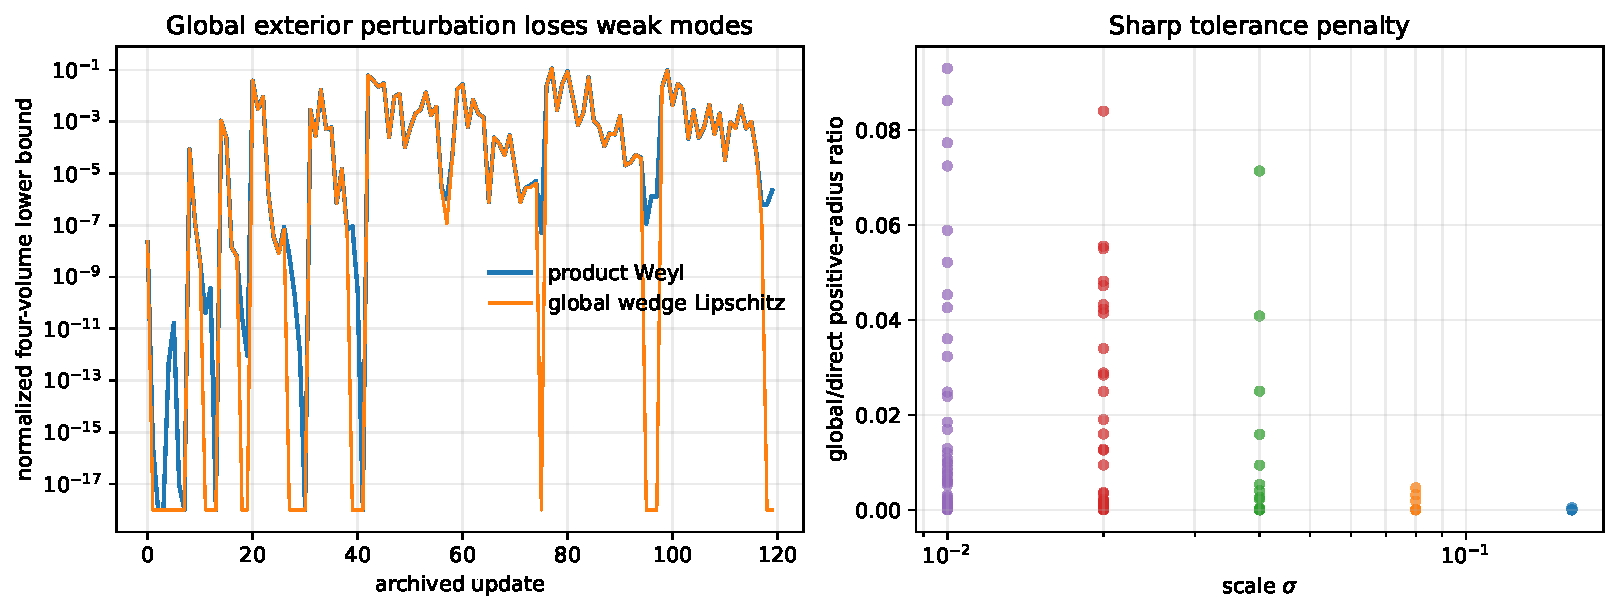
\includegraphics[width=\textwidth]{figures/global_wedge_lipschitz_barrier.pdf}
\caption{Left: product Weyl dominates the global wedge-Lipschitz lower bound
on every archived update.  Right: the global method tolerates only a fraction
of the tail radius admitted by the weak singular mode.}
\label{fig:audit}
\end{figure}

\section{Route consequence and claim boundary}
This negative result is constructive.  It identifies exactly why the global
shortcut fails and which information was discarded.  RH-113 should freeze
the recent top-four right singular frame and propagate only its four
directional images.  Such a determinant remains a lower bound for the full
exterior norm but no longer charges every error direction at $s_1$.

What is proved is the sharp global wedge law, universal Weyl domination, and
the exact positivity radius.  What is not proved is a directional wedge
bound, an all-level physical four-volume law, uniform Stage A, a
Hilbert--Polya operator, identification of zeta zeros, or the Riemann
Hypothesis.  The phrase ``negative result'' applies only to the global
norm-only branch.

\bibliographystyle{plainnat}
\bibliography{references}
\end{document}
